% Figure 4: Corridor Ray-Casting & Safe Heading Selection (TikZ Diagram)
\begin{figure}[!t]
\centering
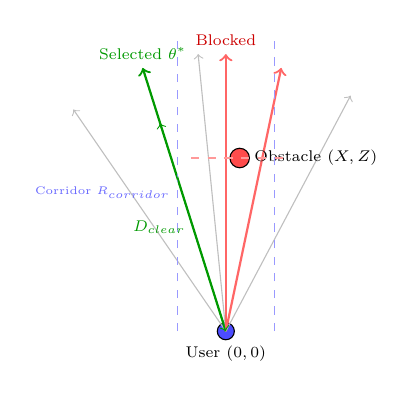
\begin{tikzpicture}[scale=0.88, every node/.style={scale=0.80}]
    % User at Origin
    \draw[fill=blue!70] (0, 0) circle (3.5pt);
    \node[below, font=\scriptsize] at (0, -0.1) {User $(0, 0)$};

    % Candidate Rays
    \draw[->, gray!50] (0, 0) -- (-2.2, 3.2);
    \draw[->, green!60!black, thick] (0, 0) -- (-1.2, 3.8) node[above, font=\scriptsize] {Selected $\theta^*$};
    \draw[->, gray!50] (0, 0) -- (-0.4, 4.0);
    \draw[->, red!60, thick] (0, 0) -- (0, 4.0) node[above, font=\scriptsize, red!80!black] {Blocked};
    \draw[->, red!60, thick] (0, 0) -- (0.8, 3.8);
    \draw[->, gray!50] (0, 0) -- (1.8, 3.4);

    % Obstacle on Center Path
    \draw[fill=red!70] (0.2, 2.5) circle (4pt);
    \node[right, font=\scriptsize] at (0.3, 2.5) {Obstacle $(X, Z)$};
    \draw[dashed, red!40] (-0.5, 2.5) -- (0.9, 2.5);

    % Safe Corridor Bounds
    \draw[dashed, blue!40] (-0.7, 0) -- (-0.7, 4.2);
    \draw[dashed, blue!40] (0.7, 0) -- (0.7, 4.2);
    \node[left, blue!60, font=\tiny] at (-0.7, 2.0) {Corridor $R_{\text{corridor}}$};

    % Clearance Vector
    \draw[<->, green!60!black] (0, 0) -- (-0.95, 3.0) node[midway, left, font=\scriptsize] {$D_{\text{clear}}$};
\end{tikzpicture}
\caption{Corridor ray-casting for local collision avoidance: angular candidate rays evaluate forward geometric clearance to arbitrate safe evasion heading $\theta^*$.}
\label{fig:corridor_raycasting}
\end{figure}
